\documentclass[../main.tex]{subfiles}

\graphicspath{{../images/}}

\begin{document}
\pagestyle{fancy}
\lhead{Lecture 15: 10/22/24}
\chead{Chapter 5}
\rhead{PHYS 421}

\section{Magnetostatics}
\barh \vspace{1em}

\paragraph{In class demonstration} Two parrell wires connected to high voltage source:
\begin{itemize}
    \item Parallel current: The wires move towards each
    \item Antiparallel current: The wires move away from each other
\end{itemize}
This implies some sort of force acting on each wire which cannot not be explained by the electrostatics we have covered thus far\dots

\subsection{Lorentz Force Law}

\begin{align*}
        \vb F_\text{mag} = Q (\vb v \cross \vb B)
\end{align*}
where $Q$ and $\vb v$ describe the moving test charge.
Compared to the force of the electric field
\begin{align*}
    \vb F_\text{elec} = Q \vb E
\end{align*}
Thus the total force is give by the Lorentz Force Law
\begin{align*}
    \boxed{
        \vb F_\text{tot} = Q(\vb E + \vb v \cross \vb B)
    }
\end{align*}
\subsubsection{Magnetic Fields}

Skip discussion so we can move straight to

\subsubsection{Magnetic Forces}
\paragraph{Cyclotron motion}

A $\vb B$ field is place into to page, and a test charge has velocity $\vb v$ moving up on the $y$-axis:
So using the right-hand-rule (RHR) the force from the magnetic field points to the left with magnitude
\begin{align*}
    F_\text{mag} = qvB = \text{acceleration} = \frac{mv^2}{R}
\end{align*}
where we have a circular motion similar to large masses rotating under gravity i.e. the ``cylotron'' radius 
\begin{align*}
    R = \frac{mv}{qB}
\end{align*}

\paragraph{Cycloid motion}

Add an $\vb E \perp \vb B \dots \vb B = B \vu x \quad \vb E = E \vu z$ 

The velocity of the test charge is given by
\begin{align*}
    \vb v = \qt(0, \dv{y(t)}{t}, \dv{z(t)}{t}) = (0, \dot y, \dot z)
\end{align*}
Where the charge is constrained in the $yz$ plane. The math says
\begin{align*}
    \vb v \cross \vb B = \begin{vmatrix}
        \vu x & \vu y & \vu z \\
        0 & \dot y & \dot z \\
        B & 0 & 0
    \end{vmatrix}
    = B \dot z \vu y - B \dot y \vu z
\end{align*}
So the force is
\begin{align*}
    \vb F &= q(\vb E + \vb v \cross \vb B) \\
    &=q (E \vu z + B \dot z \vu y) = m\vb a = m (\ddot y \vu y + \ddot z \vu z)
\end{align*}
This gives us the equations of motion
\begin{align*}
    q B \dot z &= m \ddot y \\
    q E - qB \dot y &= m \ddot z
\end{align*}
And using the ``cyclotron frequency''
\begin{align*}
    \omega \equiv \frac{qB}{m} \quad \sim \qty{}{\frac{C.T}{kg}} \sim \qty{}{\frac{rad}{s}}
\end{align*}
We can rewrite the equations of motion as
\begin{align*}
    \ddot y &= \omega \dot z \\
    \ddot z &= \omega \qt(\frac{E}{B} - \dot y)
\end{align*}
Which we can solve with the general solution
\begin{align*}
    y(t) &= C_1 \cos(\omega t) + C_2 \sin(\omega t) + \frac{E}{B}t + C_3 \\
    z(t) &= C_2 \cos(\omega t) - C_1 \sin(\omega t) + C_4
\end{align*}
with the intial conditions
\begin{align*}
    \dot y(0) &= \dot z(0) = 0 \\
    y(0) &= z(0) = 0
\end{align*}
The solution is
\begin{align*}
    y(t) &= \frac{E}{\omega B} (\omega t - \sin(\omega t)) \\
    z(t) &= \frac{E}{\omega B} (1 - \cos(\omega t))
\end{align*}
NOTE: $v = \omega R$ so the force $F = q(E + v \cross B)$ we have a length scale
\begin{gather*}
    \frac{E}{B} \sim \omega R, \quad E \sim v \cross B, \quad v \sim E/B \\
    \boxed{R \equiv \frac{E}{\omega B}}
\end{gather*}
So the equations are simplified to
\begin{align*}
    y(t) &= R(\omega t - \sin(\omega t))  \quad z(t) &= R(1 - \cos(\omega t))\\
    (y - \omega t R)^2 = R^2 \sin^2(\omega t) \quad (z - R)^2 &= R^2 \cos^2(\omega t)
\end{align*}
thus
\begin{align*}
    R^2 (c^2 + s^2) = R^2 = (z - R)^2 + (y - \omega t R)^2
\end{align*}
Since
\begin{align*}
    \dot y = v = \omega R = \frac{E}{B} 
\end{align*}
and the equation is similar to the circle $x^2 + y^2 = R^2$ so the motion is a cycloid.
So we can imagine the motion of the charge as rolling a circle along the $y$ axis! [insert cycloid path]

NOTE:
\begin{align*}
    \boxed{\textbf{magnetic fields do no work}}
\end{align*}
As a charge $q$ moves $\dd{l} = \vb v \dd{t}$ the change in word is
\begin{align*}
    \dd{\omega_\text{mag}} = \vb F_\text{mag} \cdot \dd{\vb l} = q(\vb v \cross \vb B) \cdot \vb v \dd{t} = 0
\end{align*}
But why did the wires move in the demonstration?

\subsubsection*{Currents}
We usually define the current direction $I$ using a positive charge (conventional current) because the the negative charge moving in the opposite direction of the positive charge is equivalent i.e.
\begin{align*}
    q_+ v_+ = (-q)(-v_+)
\end{align*}
The current is charge/time
\begin{align*}
    I \sim \qty{}{C/s} \sim \qty{}{A}
\end{align*}
The the line charge has current
\begin{align*}
    \vb I = \lambda \vb v \sim \qty{}{C/m.m/s} = \qty{}{A/m}
\end{align*}
In a neutral wire (or in general)
\begin{align*}
    I = \lambda_+ v_+ + \lambda_- v_-
\end{align*}
The force on a current carrying wire:
\begin{align*}
    F_\text{mag} &= \int (\vb v \cross \vb B) \dd{q} = \int (\vb v \cross \vb B) \lambda \dd{l} \\
    &= \int (\vb I \cross \vb B) \dd{l} = \int I(\dd{\vb l} \cross \vb B)
\end{align*}
where we assume that the current is constant \textit{usually} so
\begin{align*}
    \boxed{
        F_\text{mag} = I \int (\dd{\vb l} \cross \vb B)
    }
\end{align*}
% insert fig5_9.png

\paragraph{Example:}
\begin{figure}[ht]
    \centering
    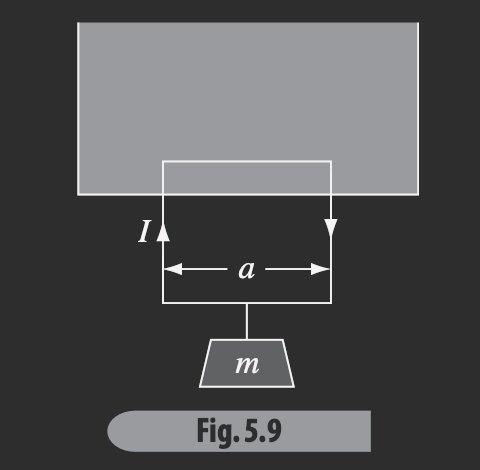
\includegraphics[width=0.5\textwidth]{fig5_9.png}
    \caption{Magnetic field above point into page}
    \label{fig:fig5_9}
\end{figure}
The current will move clockwise in the loop because on the top side in order to have the force point upwards to counteract the mass.
The force on the sides of the loop will cancel out, so the magnitude is
\begin{align*}
    \abs{\vb F_\text{mag}} = I a B = mg
\end{align*}
Now increasing $I$ will increase the force which means the whole wire move upwards with velocity $\vb u$ and a change in height $\delta h = u \delta t$.
This now looks like work
\begin{align*}
    \delta W_\text{mag} = I a B \delta h
\end{align*}
Who is doing the work to keep lifting the wire? The battery!
This is analogous to normal force on applying force to a mass on an incline;
the normal force does no work, but only redirects the force upwards. So magnetic force is like the normal force.

\lhead{Lecture 16: 10/24/24}

\paragraph{Surface Current Density} When charge flows on a surface, this density
\begin{align*}
    \vb K \equiv \dv{\vb I}{l_\perp}
\end{align*}
where we can image $l_\perp$ as a thin ribbon (\ref{fig:fig5_12}) and $K$ is the current per unit width thus
\begin{align*}
    \vb K = \sigma \vb v
\end{align*}

% fig5_12.png
\begin{figure*}[ht]
    \centering
    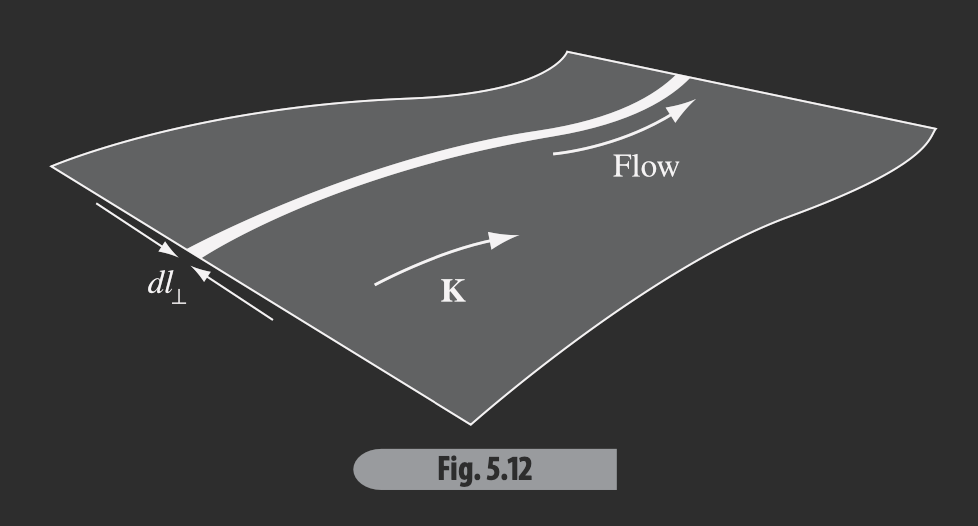
\includegraphics[width=0.4\textwidth]{fig5_12.png}
    \caption{Surface current density}
    \label{fig:fig5_12}
\end{figure*}

\paragraph{Magnetic force in 2D} From the 1D $\vb F_\text{mag} = I \int \dd{\vb l} \cross \vb B$, so for 2D
\begin{align*}
    \vb F_\text{mag} = \int (\vb v \cross \vb B) \sigma \dd{a} = \int (\vb K \cross \vb B) \dd{a}
\end{align*}

\paragraph{For a charge dist. in a volume}
\begin{align*}
    \vb J \equiv \frac{\vb I}{a_\perp} \sim \text{current/unit area}
\end{align*}

% fig5_13.png
\begin{figure*}[ht]
    \centering
    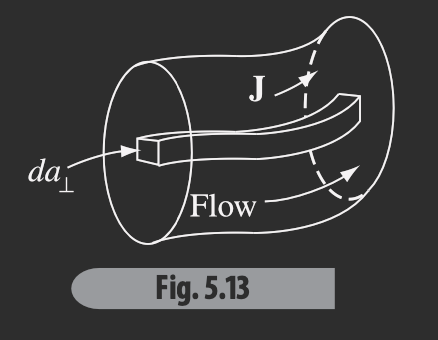
\includegraphics[width=0.4\textwidth]{fig5_13.png}
    \caption{Volume current density}
    \label{fig:fig5_13}
\end{figure*}

So we can find this (mobile) volume charge density with
\begin{align*}
    \vb J = \rho \vb v
\end{align*}
Think of this steady current as a column of water moving along this pipe.
Rather than looking at each individual water molecule, we can look at the flow of the water as a whole.

In a $\vb B$ field there is a force
\begin{align*}
    \vb F_\text{mag} = \int (\vb v \cross \vb B) \rho \dd{\tau} = \int (\vb J \cross \vb B) \dd{\tau}
\end{align*}
With current $I$ \& uniform cross-sectional area (a wire), the volume charge density is
\begin{align*}
    \vb J = \frac{I}{\pi a^2}
\end{align*}

\begin{figure*}
    \centering
    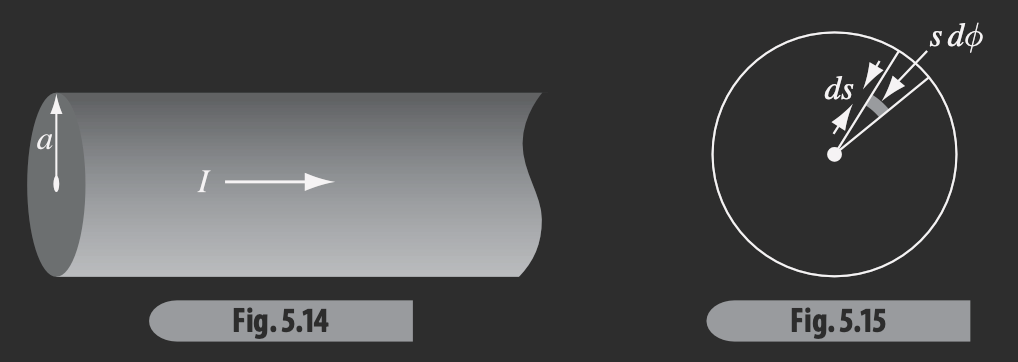
\includegraphics[width=0.6\textwidth]{fig5_14_15.png}
    \caption{Volume current density}
    \label{fig:fig5_14}
\end{figure*}

With $J \propto$ distance from the center of the wire thus
\begin{align*}
    J = ks, \quad k\sim \text{constant}
\end{align*} 
The current is 
\begin{align*}
    I &= \int \dd{I} = \int \vb J \cdot \dd{\vb a_\perp} \\
    &= \int (ks) s \dd{s} \dd(\phi) \\
    &= 2\pi k \int_0^a s^2 \dd{s} = 2\pi k \frac{a^3}{3}
\end{align*}

\paragraph{Total current crossing a surface}
\begin{align*}
    I = \int_S J \dd{\vb a_\perp} = \int_S \vb J \cdot \dd{\vb a_\perp}
\end{align*}
If the surface is \textit{closed}: 
if there is a source inside the surface, there is a net flow coming out of the surface and vice versa.
\begin{align*}
    \oint_S \vb J \cdot \dd{\vb a} = -\dv{t} \int_V \rho \dd{\tau} = - \int_V \qt(\dv{\rho}{t}) \dd{\tau}
\end{align*}
From the divergence theorem
\begin{align*}
    \oint_S \vb J \cdot \dd{\vb a} = \int_V (\div{\vb J}) \dd{\tau}
\end{align*}
or also known as the ``continuity equation''
\begin{align*}
    \boxed{
        \div{\vb J} = -\pdv{\rho}{t}
    }
\end{align*}
\newpage
\subsection{Biot-Savart Law}
\begin{itemize}
    \item Stationare charge $\to$ const. $\vb E \to$ electrostatics (Coloumbs Law)
    \item Steady currents $\to$ const. $\vb B \to$ magnetostatics (Biot-Savart Law)
\end{itemize}

\subsubsection{Steady Currents}
ASSUME
\begin{align*}
    \pdv{\rho}{t} = 0 \implies \pdv{\vb J}{t} = 0
\end{align*}
For most technologies, computers, etc.
\begin{itemize}
    \item freq $\to \sim$ 10-100 MHz; which is fast and reaches a limit due to the speed of light\dots (lets not worry about this for now)
\end{itemize}
% fig5_16.png
\begin{figure*}[ht]
    \centering
    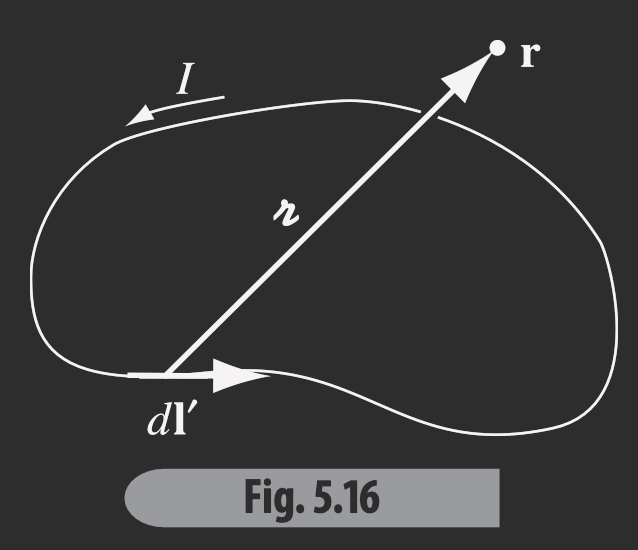
\includegraphics[width=0.4\textwidth]{fig5_16.png}
    \caption{Biot-Savart Law along a wire}
    \label{fig:fig5_16}
\end{figure*}

The $\vb B$ field of a steady current line currents is
\begin{align*}
    \vb B(\vb r) &= \frac{\mu_0}{4\pi} \int \frac{\vb I \cross \vu{\scriptr}}{\scriptr^2} \dd{l'} \\
    &= \frac{\mu_0}{4\pi} I \int \frac{\dd{\vb l'} \cross \vu{\scriptr}}{\scriptr^2}
\end{align*}
where we integrate along the current path and $\mu_0$ is the permeability of free space
\begin{align*}
    \mu_0 \approx 4\pi \times 10^{-7} \qty{}{\frac{N}{A^2}}
\end{align*}
Units of magnetic field:
\begin{align*}
    B \sim \qty{}{\frac{N}{A.m}} \sim \qty{}{\frac{V.s}{m^2}} \sim T \to \text{Tesla}
\end{align*}
Where the Earth has a magnetic field of a few $\mu$ T compared to a NMR machine which has a field of a few T.

\newpage
\paragraph{Example:} Find $\vb B$ field a distance $s$ from a long striaght current carrying wire $I$.

% fig5_17_18.png
\begin{figure*}[ht]
    \centering
    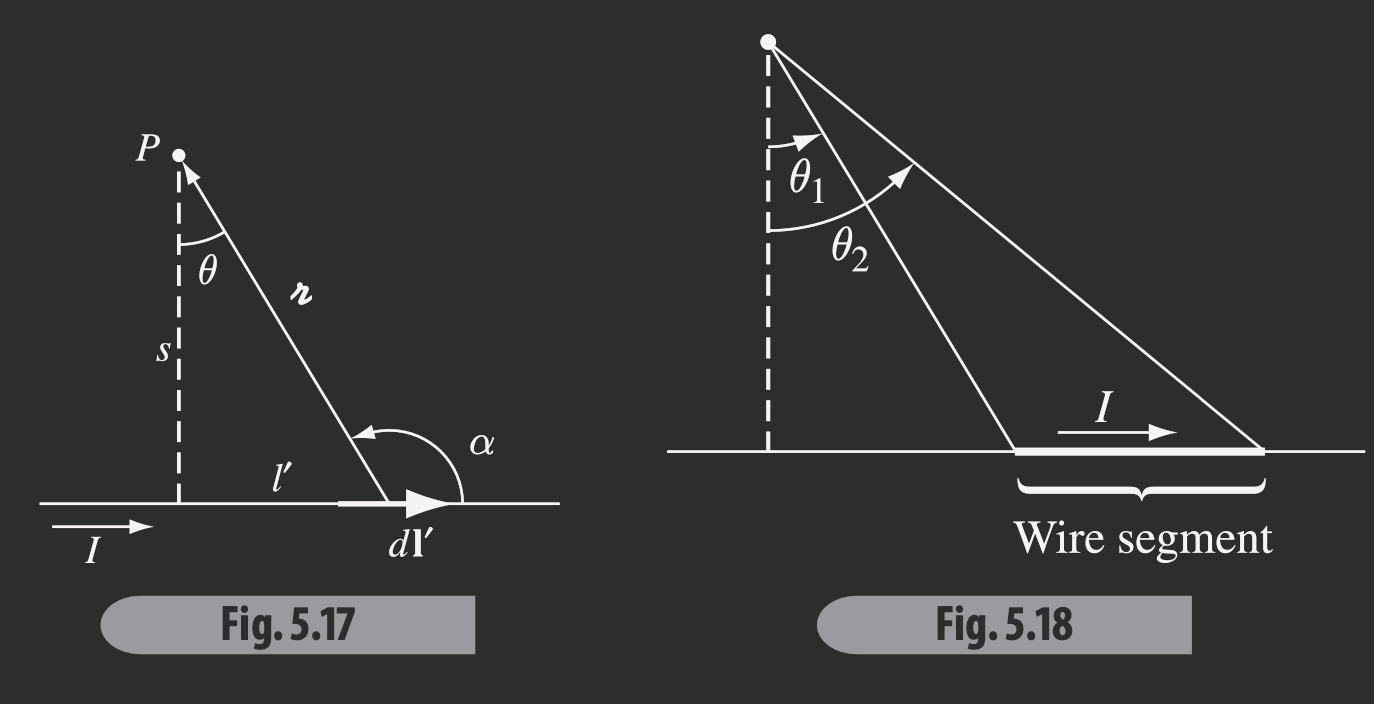
\includegraphics[width=0.8\textwidth]{fig5_17_18.png}
    \caption{B-field a disance along a wire}
    \label{fig:fig5_17}
\end{figure*}

From the Biot-Savart Law
\begin{align*}
    \vb B (\vb r) = \frac{\mu_0}{4\pi} I \int \frac{\dd{\vb l'} \cross \vu{\scriptr}}{\scriptr^2}
\end{align*}
So looking at each part:
\begin{itemize}
    \item $\dd{\vb l' \cross \vu{\scriptr}}$ at P tells us $\vb B \sim (-\vu y)$ (RHR)
    with magnitude
    \begin{align*}
        \dd{l'} \sin\alpha = \dd{l'} \cos\theta
    \end{align*}
    \item $l' = s\tan\theta$ so
    \begin{align*}
        \dd{l'} = s \sec^2\theta \dd{\theta}
    \end{align*}
    \item $s = \scriptr \cos\theta$ so 
    \begin{align*}
        \frac{1}{\scriptr^2} = \frac{\cos^2\theta}{s^2}
    \end{align*}
\end{itemize}
\newpage
Thus
\begin{align*}
    \abs{\vb B} &= \frac{\mu_0 I}{4\pi} \int_{\theta_1}^{\theta_2} \frac{\cos\theta}{s} \dd{\theta} \\
    &= \frac{\mu_0 I}{4\pi s} \int_{-\pi/2}^{\pi/2} \cos\theta \dd{\theta} = \frac{\mu_0 I}{2\pi s}
\end{align*}
We can imagine this as a circle around the wire capturing this B-field or wrapping your fingers around the wire where the thumb point in the direction of the current (RHR).

% figure finger.png
\begin{figure*}[ht]
    \centering
    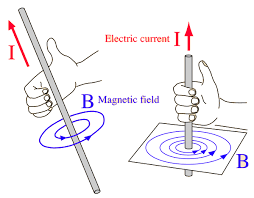
\includegraphics[width=0.4\textwidth]{finger.png}
    \caption{Right-hand rule}
    \label{fig:finger}
\end{figure*}

\paragraph{Back to demo}
% fig5_19.png
\begin{figure*}[ht]
    \centering
    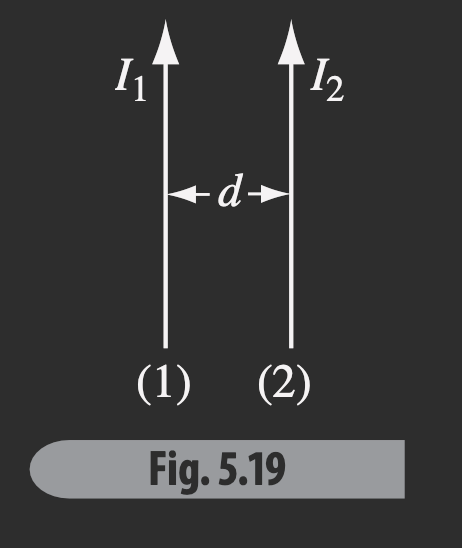
\includegraphics[width=0.4\textwidth]{fig5_19.png}
    \caption{Demo}
    \label{fig:fig5_19}
\end{figure*}
We can now see the forces on the wires due to each other's magnetic fields.

\newpage 
\lhead{Lecture 17: 10/29/24}

\subsection{Divergence and Curl of B}
\subsubsection{Straight Line Currents}
Integrating $\vb B$ around a circle of radius $s$ for a long straight wire:
\begin{align*}
    &\oint \vb B \cdot \dd{\vb l} \quad \vb B = \frac{\mu_0 I}{2\pi s} \vu*\phi \\
    &= \oint \frac{\mu_0 I}{2\pi s} s \dd{\phi} = \mu_0 I
\end{align*}
which is independent of $s$!

Even for any loop around the wire $\dd{\vb l} = \dd{s} \vu*{s} + s \dd{\phi} \vu*{\phi} + \dd{z} \vu{z}$ so
\begin{align*}
    \oint \vb B \cdot \dd{\vb l} = \int \frac{\mu_0 I}{2\pi s} s \dd{\phi} = \mu_0 I
\end{align*}
For a bundle of straight wires,
\begin{align*}
    \oint \vb B \cdot \dd{\vb l} = \mu_0 I_\text{enc}
\end{align*}
From our intuitin we can use the divergence theorem to get
\begin{align*}
    \oint \vb B \cdot \dd{\vb l} = \in (\curl \vb B) \cdot \dd{\vb a} = \mu_0 I = \mu \int \vb J \cdot \dd{\vb a}
\end{align*}
or ``Ampere's Law''
\begin{align*}
    \boxed{
        \curl \vb B = \mu_0 \vb J
    }
\end{align*}

\subsubsection{Divergence and Curl of B}
\paragraph{How about div of B?}
\begin{align*}
    \vb B (\vb r) = \frac{\mu_0}{4\pi} \int \frac{\vb J (\vb r') \cross \vu*{\scriptr}}{\scriptr^2} \dd{\tau'}
\end{align*}
so 
\begin{align*}
    \div \vb B = \frac{\mu_0}{4\pi} \int \div \qt(\vb J \cross \frac{\vu*{\scriptr}}{\scriptr^2}) \dd{\tau'}
\end{align*}
where the quantity in the integral is
\begin{align*}
    \frac{\vu*{\scriptr}}{\scriptr^2} \cdot (\curl \vb J) - \vb J \qt(\curl \frac{\vu*{\scriptr}}{\scriptr^2}) = 0 
\end{align*}
this is proved in Griffiths Prob 1.63\dots anyways this tells us
\begin{align*}
    \boxed{
        \div \vb B = 0
    }
\end{align*}

\subsubsection{Ampere's Law}
Again
\begin{align*}
    \curl \vb B = \mu_0 \vb J
\end{align*}
where
\begin{align*}
    \in (\curl \vb B) \cdot \dd{\vb a}  = \oint \vb B \cdot \dd{\vb l} = \mu \int \vb J \cdot \dd{\vb a} = \mu_0 I_\text{enc}
\end{align*}
thus
\begin{align*}
    \boxed{
        \oint \vb B \cdot \dd{\vb l} = \mu_0 I_\text{enc}
    }
\end{align*}
for a current enclosed by an ``Amp\`erian oop''

\paragraph{Example:} The magnetic field of a long straight wire with steady current $I$ is
\begin{align*}
    &\oint B \cdot \dd{\vb l} = B \int s \dd{\phi} = B 2\pi s = \mu I_\text{enc} \\
    &\implies B = \frac{\mu_0 I}{2\pi s} \vu*{\phi}
\end{align*}
which is easier to get to compared to the last time we did this.

\paragraph{Example:} Find $\vb B$ due to infinite uniform surface current $\vb K = K_0 = \vu x$:

Drawing an amperian loop as a rectangle perpendicular to current above and below the current sheet: $\dd{\vb l} = 2 B l$ and
\begin{align*}
    I_\text{enc} = K_0 l
\end{align*}
so
\begin{align*}
    B = \frac{\mu_0 K_0}{2}
\end{align*}

\paragraph{Example:} An infinitely long solenoid\dots using an amperian loop: a rectangle around the middle of the solenoid and outside it.
\begin{align*}
    2Bl = \mu_0 I (n l)
\end{align*}
but we can make the loop outside the solenoid go infinitely far away so
\begin{align*}
    Bl = \mu_0 n I l
\end{align*}
or the classic result
\begin{align*}
    \boxed{
        B = \mu_0 n I
    }
\end{align*}

\newpage
\lhead{Lecture 18: 10/31/24}

\subsection{Magnetic Vector Potential}

\subsubsection*{The Vector Potential}
From the divergence of $\vb B$ we introduce a vector potential of the magnetic field such that
\begin{align*}
    \div \vb B = 0 \implies \div (\curl \vb V) = 0
\end{align*}
so we define
\begin{align*}
    \boxed{
        \vb B = \curl \vb A
    }
\end{align*}
and from Ampere's Law
\begin{align*}
    \curl \vb B = \mu_0 \vb J = \curl (\curl \vb A) = \grad (\div \vb A) - \laplacian \vb A
\end{align*}
In electrostatics we had
\begin{align*}
    \vb E = - \grad V \quad V \to V + C \qqtext{``gauge freedom''}
\end{align*}
where ``gauge freedom'' is a fancy way of saying we can add a constant to the potential and it won't change the physics.

Similarly for $\vb B$:
\begin{align*}
    \curl \grad F = 0 
\end{align*}
where we want to make 
\begin{align*}
    \div A \to 0
\end{align*}
Method: Say we have a potential $\vb A_0$ where $\vb B_0 = \curl \vb A_0$ i.e.
\begin{align*}
    \vb A_0 \to \vb A + \grad \lambda \equiv \vb A
\end{align*}
Thus
\begin{align*}
    \vb B = \curl A = \curl (\vb A_0 + \grad \lambda) = \curl \vb A_0 + 0 = \vb B_0
\end{align*}
but we know that
\begin{align*}
    \div \vb A = \div \vb A_0 + \underbrace{\div(\grad \lambda)}_{\laplacian \lambda}= 0, \quad 
\end{align*}
So we get $\div \vb A \if \laplacian \lambda = - \div \vb A_0$. To find this $\lambda$ we can you the same Poisson's equation method like in electrostatics.

$\implies$ From electrostatics:
\begin{align*}
    \laplacian V = -\frac{\rho}{\epsilon_0} \to V = \ke \int \frac{\rho}{\scriptr} \dd{\tau'}
\end{align*}
So for magnetostatics
\begin{align*}
    \lambda = \frac{1}{4\pi} \int \frac{\div \vb A_0}{\scriptr} \dd{\tau'}
\end{align*}

Why did we do all this?

$\implies$ All for Amp\`er's law:
\begin{align*}
    \curl \vb B = -\laplacian \vb A = \mu_0 \vb J
\end{align*}
where we fnially get
\begin{align*}
    \boxed{
        \laplacian \vb A = -\mu_0 \vb J
    }
\end{align*}
Now we can just find the vector potential from a current distribution
\begin{align*}
    \vb A (\vb r) = \frac{\mu_0}{4\pi} \int \frac{\vb J (\vb r)}{\scriptr} \dd{\tau'}
\end{align*}
which is a much easier way to find the magnetic field rather than our previous Bio-Savart Law which had a curl inside the integral!
for line and sheet currents
\begin{align*}
    \to \int \frac{\vb I}{\scriptr} \dd{l'} \quad \int \frac{\vb K}{\scriptr} \dd{a'}
\end{align*}

Before we tackle this example heavy in math, we recommend reading the Feynmane lectures \href{https://www.feynmanlectures.caltech.edu/}{Website}.
\paragraph{Example} A spherical shell, radius, $R$, uniform fixed surface charge $\sigma$ set to spin at $\vb \omega$. Find $\vb A(\vb r)$

% fig5_48_49.png
\begin{figure*}[ht]
    \centering
    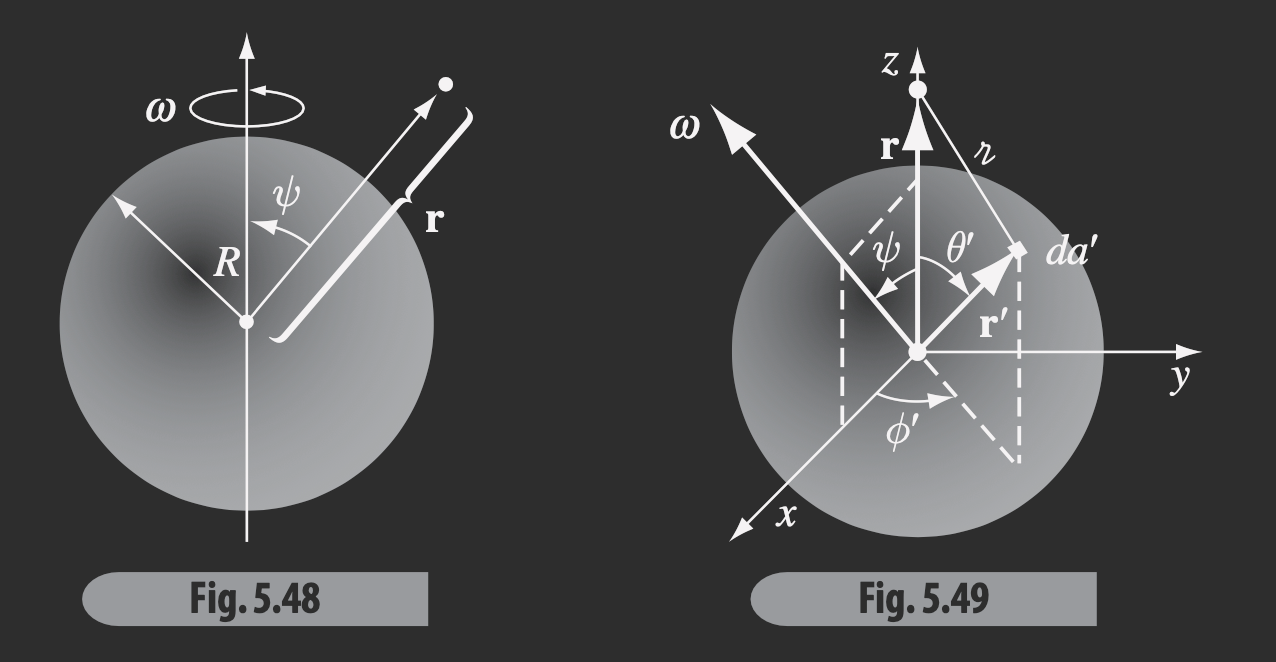
\includegraphics[width=0.8\textwidth]{fig5_48_49.png}
    \caption{All the components}
    \label{fig:fig5_48}
\end{figure*}
All the stuff we need:
\begin{itemize}
    \item The vector potential
    \begin{align*}
        \vb A (\vb r) = \frac{\mu_0}{4\pi} \int \frac{\vb K (\vb r')}{\scriptr} \dd{a'}
    \end{align*}
    \item With current density $\vb K = \sigma \vb v$ and separation vector $\vb \scriptr = \vb r - \vb r'$ with magnitude
    \begin{align*}
        \scriptr = \sqrt{R^2 + r'^2 - 2Rr' \cos\theta}
    \end{align*}
    \item The area element
    \begin{align*}
        \dd{a'} = R^2 \sin\theta' \dd{r'} \dd{\theta'} \dd{\phi'}
    \end{align*}
    and from position vector
    \begin{align*}
        \vb r' = R(\sin\theta' \cos\phi', \sin\theta' \sin\phi', \cos\theta')
    \end{align*}
    \item The velocity
    \begin{align*}
        \vb v &= \vb \omega \cross \vb r' = R \begin{vmatrix}
            \vu x & \vu y & \vu z \\
            \omega \sin\theta' & 0 & \omega \cos\theta' \\
            \sin\theta' \cos\phi' & \sin\theta' \sin\phi' & \cos\theta'
        \end{vmatrix} \\
        &= \omega R \qt[
            -(\cos\psi \sin\theta' \sin\phi') \vu x
            + (\cos\psi \sin\theta' \cos\phi' - \sin\psi \cos\theta') \vu y
            + (\sin\psi \sin\theta' \sin\phi') \vu z
        ]
    \end{align*}
    We do this so that any terms including $\sin\phi'$ or $\cos\phi'$ will integrate to zero:
    \begin{align*}
        \int_0^{2\pi} \sin\phi' = \int_0^{2\pi} \cos\phi' \dd{\phi'} = 0
    \end{align*}
    So we can a much simpler
    \begin{align*}
        \vb v = -\omega R \qt[
            \sin\psi \cos\theta' \vu y
        ]
    \end{align*}
\end{itemize}
Thus we have 
\begin{align*}
    \vb A (\vb r) = \frac{\mu_0}{4\pi} \sigma (-\omega R \sin\psi) R^2 2\pi \vu y
    \int_0^\pi \frac{\cos\theta'\sin\theta'}{\sqrt{R^2 + r^2 - 2Rr\cos\theta'}} \dd{\theta'}
\end{align*}
after integration with substitution\dots we have two results
\begin{itemize}
    \item If $\abs{\vb r} < R$ the integral goes to
    \begin{align*}
        \int \to \frac{2r}{3R^2}
    \end{align*}
    \item If $\abs{\vb r} > R$ the integral goes to
    \begin{align*}
        \int \to \frac{2R}{3r^2}
    \end{align*}
    We can see that
    \begin{align*}
        \vb*\omega \cross \vb r = (-\omega R \sin\psi) \vu y
    \end{align*}
    which will transform our tilted form to the original form (Fig. \href{fig:fig5_48}).

    Finally
    \begin{align*}
        \vb A (\vb r) = \begin{cases}
            \frac{\mu_0 R \sigma}{3} (\vb*\omega \cross \vb r) & \text{Inside sphere} \\
            \frac{\mu_0 R^4 \sigma}{3r^2} (\vb*\omega \cross \vb r) & \text{Outside sphere}
        \end{cases}
    \end{align*}
    And letting $\vb*\omega \propto \vu z$, and $\vb r$ at $(r, \theta, \phi)$:
    \begin{align*}
        \vb A (r, \theta, \phi) = \begin{cases}
            \frac{\mu_0 R \sigma}{3} \omega r \sin\theta \vu \phi & \text{Inside sphere} \\
            \frac{\mu_0 R^4 \sigma}{3r^2} \omega r \sin\theta \vu \phi & \text{Outside sphere}
        \end{cases}
    \end{align*}
    Thus the magnetic field in side the sphere is
    \begin{align*}
        \vb B(\abs{\vb r} < R) = \curl \vb A = \frac{2}{3} \mu_0 R \sigma \omega \vu{z}
    \end{align*}
    Suprisingly a uniform magnetic field!
\end{itemize}
Or (from Feynman) a sphere with wire wrapped around it like a solenoid.

\newpage
\subsubsection{Multipole Expansion}
Recalling what we did for the electric field
\begin{align*}
    \frac{1}{\scriptr} = \frac{1}{r} \sum_{n = 0}^\infty \qt(\frac{r'}{r})^n P_n (\cos\alpha)
\end{align*}
\begin{figure*}[ht]
    \centering
    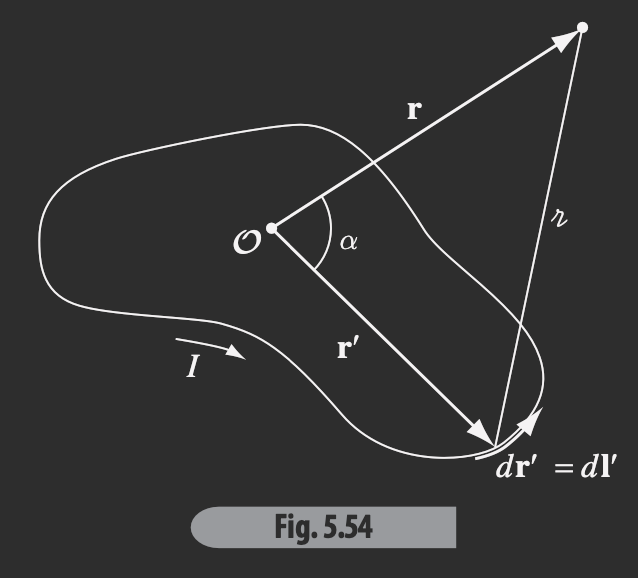
\includegraphics[width=0.4\textwidth]{fig5_54.png}
    \caption{Field point $P$ for loop of line current}
    \label{fig:5_54}
\end{figure*}

For the line charge, the vector potential is
\begin{align*}
    \vb A (\vb r) &= \frac{\mu_0 I}{4\pi} I \int \frac{\dd{\vb l'}}{\scriptr} \\
    &= \frac{\mu_0 I}{4\pi} \sum_{n = 0}^\infty \frac{1}{r^{n+1}} \oint (r')^n P_n (\cos\alpha) \dd{\vb l'} \\
    &= \frac{\mu_0 I}{4\pi} \qt[
        \underbrace{\cancel{\frac{1}{r} \oint \dd{\vb l'}}}_{\text{mono}} 
        + \underbrace{\frac{1}{r^2} \oint r' \cos\alpha \dd{\vb l'}}_{\text{dipole}}
        + \underbrace{\frac{1}{r^3} \oint (r')^2 P_2 (\cos\alpha) \dd{\vb l'}}_{\text{quadrupole}}
        + \dots
    ]
\end{align*}
Where we can see that the monopole term is zero as magnetic monopoles do not exist.
Looking at the dipole term
\begin{align*}
    \vb A_\text{dip} (\vb r) &= \frac{\mu_0 I}{4\pi r^2} \oint r' \cos\alpha \dd{\vb l'}
\end{align*}
where the integral has $\vu r \cdot \vb r'$ so
\begin{align*}
    \oint (\vu r \cdot \vb r) \dd{\vb l'} = - \vu r \cross \int \dd{\vb a'} = \int \dd{\vb a'} \cross \vu r
\end{align*}
This gives us
\begin{align*}
    \vb A_\text{dip} (\vb r) = \frac{\mu_0 I}{4\pi r^2}  \vb m \cross \vu r
\end{align*}
where
\begin{align*}
    \vb m = I \int \dd{\vb a'}
\end{align*}
The field lines rather go through the loop and because we have no monopole term.
\end{document}